\documentclass[a4paper,10pt]{article}
\usepackage[colorlinks = true,
            linkcolor = blue,
            urlcolor  = blue,
            citecolor = blue,
            anchorcolor = blue]{hyperref}
\usepackage{graphicx}
\usepackage{url}
\usepackage{listings}
\newcommand\tab[1][0.5cm]{\hspace*{#1}}

% Title Page
\title{Scikit Learn}
\author{Nagy Lilla}


\begin{document}
\maketitle


\tableofcontents
\section{Overview}

\tab My project of choice is \href{http://scikit-learn.org/stable/auto_examples/plot_multioutput_face_completion.html#sphx-glr-auto-examples-plot-multioutput-face-completion-py}{scikit}, which is a data mining and analyzing tool using python, with many useful libraries in the field of data analysis, classification and clustering.

 \subsection{Running instructions}
\tab For installing the project, run the following commands:
\begin{lstlisting}
pip2 install numpy
pip2 install matplotlib
sudo apt-get install python-tk
pip2 install scipy
pip2 install -U scikit-learn
pip install scikit-image
\end{lstlisting}
\tab To run the \href{http://scikit-learn.org/stable/auto_examples/plot_multioutput_face_completion.html#sphx-glr-auto-examples-plot-multioutput-face-completion-py}{example} :
\begin{lstlisting}
python plot_multioutput_face_completion.py
\end{lstlisting}
 
 
 \subsection{Theoretical aspects}
  \subsubsection{Data representation}
  \tab The data is represented as a dataset, that is a dictionary-like object that holds all the data and some metadata about the data. This data is stored in the {\fontfamily{qcr}\selectfont .data} member, which is an {\fontfamily{qcr}\selectfont n\_samples}, {\fontfamily{qcr}\selectfont n\_features} 2D array, regardless of the shape of the original data.
  \subsubsection{Algorithm}
\tab There are two learning methods: \textbf{supervised learning} and \textbf{unsupervised learning}. \\
\tab \textbf{Supervised learning} contains additional attributes that we want to predict. This can be either \textbf{classification} or \textbf{regression}, depending whether the output is a continuous or a discrete category. \\
 \tab In \textbf{unsupervised learning}, we don't know what our target values are gonna be, so we have to do either \textbf{clustering}, or \textbf{density estimation}. \\ 
 \tab The common way to evaluate a learning algorithm is to split the data into two different sets: \textbf{training set}, on which learning is performed, and \textbf{test set}, on which we test it. \\
 \tab The whole process is performed the following way: \\ 
 \tab The program gets a dataset with certain values. On these values, an estimator has to be used, which is basically using a fitting function on the mentioned dataset, and then predicting the values of the unseen samples. This way, we get an instance of the estimator class. This estimator class will be then used on the training set together with the fit function, to predict new values. Unless other data type is specified, the results of the functions are cast to {\fontfamily{qcr}\selectfont float64}.
 
 \subsection{Existing Example}
  \tab As I mentioned before, I chose the following \href{http://scikit-learn.org/stable/auto_examples/plot_multioutput_face_completion.html#sphx-glr-auto-examples-plot-multioutput-face-completion-py}{example} for my code, with the aforementioned running instructions. \\
  \tab This example is used to fetch a set of faces, and then predict the lower half of them based on the upper half of them using different methods. This means that the faces are used as the training set and the upper halves are used as the test set to generate the lower halves of the faces.\\
  \tab Four different functions are used to perform this, for the four different methods with which faces can be estimated: 
\begin{itemize}
\item Extra trees
\item K-nn
\item Linear regression
\item Ridge
\end{itemize}
\tab These functions will result in estimators, that are gonna be used to fit on the training set, and then to predict on the test set. \\
\tab Then, the results are showed using the methods {\fontfamily{qcr}\selectfont subplot} and {\fontfamily{qcr}\selectfont imshow}. \\ 
\tab Therefore, the input is a set of images, and the output is a set of predicted images showed with the help of {\fontfamily{qcr}\selectfont matplotlib}.
  
 \subsection{Your own small Example}
 \tab My example consists of color quantization using K-Means on a picture of a raccoon, which basically reduces the number of used colors significantly, while maintaining a relatively high quality aspect. This uses color quantization with 32 colors and then outputs the original picture, the result of applying K-Means and last but not least, applying predictions randomly. We can clearly see that applying K-Means has a much better output than with random predictions, because it maintains a much better overall quality.
 \begin{lstlisting}
import numpy as np
import matplotlib.pyplot as plt
from sklearn.cluster import KMeans
from sklearn.metrics import pairwise_distances_argmin
from sklearn.utils import shuffle
from PIL import Image

n_colors = 32

# Load the raccoon image
waschbar = Image.open("waschbar.jpg")

# Convert to floats and then divide by 255 so that imshow will work on it
# (The values have to be in range [0,1])
waschbar = np.array(waschbar, dtype=np.float64) / 255

# Transform image to a 2D array
w, h, d = original_shape = tuple(waschbar.shape)
assert d == 3
image_array = np.reshape(waschbar, (w * h, d))

# Fitting the model on a small subsample of the data
image_array_sample = shuffle(image_array, random_state=0)[:1000]
kmeans = KMeans(n_clusters=n_colors, random_state=0).fit(image_array_sample)

# Predicting color indices on the full image using k-means
labels = kmeans.predict(image_array)

# Predicting color indices on the full image randomly 
random = shuffle(image_array, random_state=0)[:n_colors + 1]
labels_random = pairwise_distances_argmin(random, image_array, axis=0)


# Recreate image of a certain size using the codebood and the labels
def recreate_image(codebook, labels, w, h):
    d = codebook.shape[1]
    image = np.zeros((w, h, d))
    label_idx = 0
    for i in range(w):
        for j in range(h):
            image[i][j] = codebook[labels[label_idx]]
            label_idx += 1
    return image

# Display all results, alongside original image
plt.figure(1)
plt.clf()
ax = plt.axes([0, 0, 1, 1])
plt.axis('off')
plt.title('Original image (96,615 colors)')
plt.imshow(waschbar)

plt.figure(2)
plt.clf()
ax = plt.axes([0, 0, 1, 1])
plt.axis('off')
plt.title('Quantized image (32 colors, K-Means)')
plt.imshow(recreate_image(kmeans.cluster_centers_, labels, w, h))

plt.figure(3)
plt.clf()
ax = plt.axes([0, 0, 1, 1])
plt.axis('off')
plt.title('Quantized image (32 colors, Random)')
plt.imshow(recreate_image(random, labels_random, w, h))
plt.show()
\end{lstlisting}

\begin{figure}[h]
 \centering
  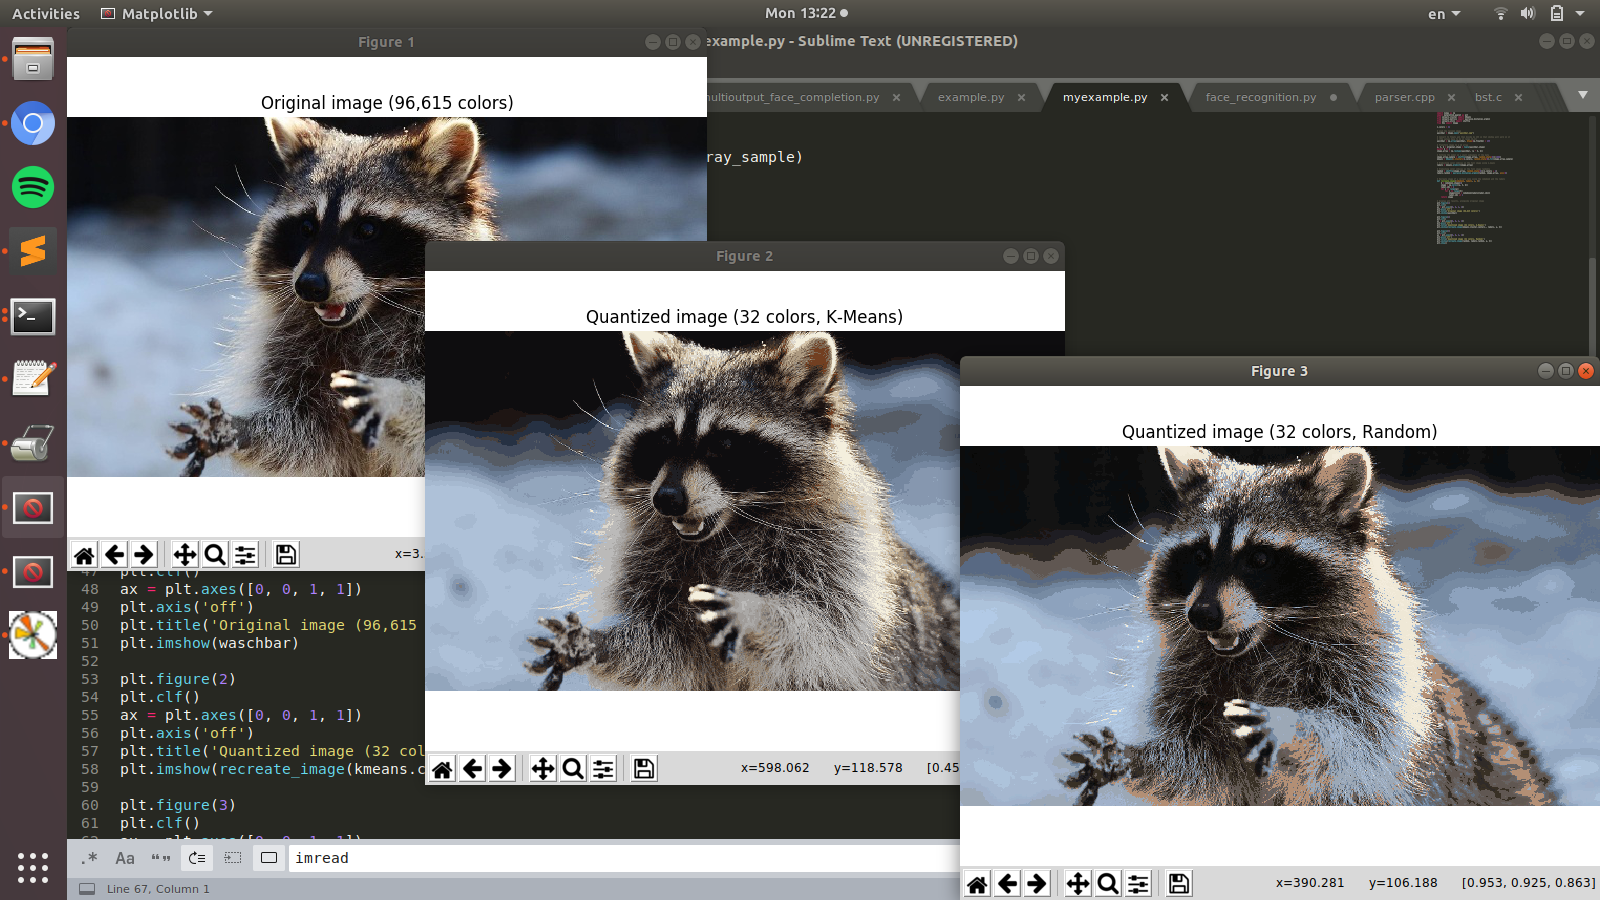
\includegraphics[width=1\textwidth]{raccoon.png}
  \caption{The output of my example}
 \end{figure}
 
 \section{Proposed problem}
  \subsection{Specification} 
  \tab Object recognition is a really important application of learning algorithms. It can be used in a really wide range of fields, from solving day-to-day problems to applying it in really important fields, such as medicine. Examples for all these applications would be getting the license plates of speeding cars on the highways, unlocking smartphones using face recognition and even applying image recognition and data processing to analyze brain tumors. \\
  \tab Therefore, my proposed problem would be to develop an object recognition program using {\fontfamily{qcr}\selectfont scikit}, which will first use a big set of data for the learning algorithm, and then test it on a test set, by also documenting the results. This way, any object category could be recognized by my program, based on the data set inputted to it. But for testing and showing the results of my program, I would select one object category, which will be used then for presenting the solution.\\
  \tab The following articles are also about using {\fontfamily{qcr}\selectfont scikit} for processing images:\\
  \tab \href{https://peerj.com/articles/453.pdf}{scikit-image: image processing in Python}\\
  \tab \href{https://link.springer.com/content/pdf/10.1186\%2Fs40679-016-0031-0.pdf}{Analyzing microtomography data with Python and the scikit-image library}\\
  
  \subsection{Implementation} 
  
  \tab In the medical field, image processing can really come in aid to doctors in helping them identify some diseases. As these diseases carry lots of similarities, they can be classified, and for this we can use artificial intelligence. \\
  \tab The main approach to do this has 3 steps:
  \begin{enumerate}
      \item Preparing the images for processing (transform them to black and white usually, normalize their contrast and resize them to the same size)
      \item Create a data set by adding labels to the images
      \item Divide the data set based on some ratio into learning set and test set
      \item Use a classifier on the learning set to group the pictures in the classes using their features
      \item Run a predictor on the test set to check how many of the results were predicted accurately
      \item Check the values and compare them based on running time and accuracy
  \end{enumerate}
  \tab In order to do this, I've used a classifier called SVC (Support Vector Classifier) from the scikit package. \\
  \tab I did the project in a few steps, starting from a much bigger data set of different pictures, at first trying to decide whether we have a raccoon on a picture or not, and then I tested the final solution on a medical data set, testing whether an eye is healthy, has glaucoma or diabetic retinopathy from the following website: \href{https://www5.cs.fau.de/research/data/fundus-images/}{https://www5.cs.fau.de/research/data/fundus-images/} \\
  \tab As main implementation I will provide the final solution that I've used for medical analysis, but in the following subsections I will explain all of the phases of the project I've tested and tried in order to get to the final solution.
  
  \begin{lstlisting}
import numpy as np
import time
from PIL import Image
from skimage import img_as_float, exposure
from sklearn import svm, metrics, model_selection
from random import shuffle
from collections import namedtuple
from sklearn.decomposition import PCA

start_time = time.time()

size = 240, 160

healthy = []
glaucoma = []
diabet = []

# read dataset into an array of images and return it
# process the images by:
# 	- converting them to black & white
# 	- resizing them to the same size (240x160)
# 	- normalize the contrast (with percentile and rescale_intensity) 
def readdataset(dataset, folder, tag, nr):
	for x in range(1,nr):
		img = Image.open('./everything/' + folder + '/' + 
		'{0:02}'.format(x) + tag + '.jpg').convert('LA')
		img = img.resize(size, 0)
		image = np.array(img)
		p2, p98 = np.percentile(image, (2, 98))
		img_rescale = exposure.rescale_intensity(image,
		in_range=(p2, p98))
		dataset.append(img_rescale)
	return dataset

# read the two datasets from file
healthy = readdataset(healthy, 'healthy', '_h', 16)
glaucoma = readdataset(glaucoma, 'glaucoma', '_g', 16)
diabet = readdataset(diabet, 'diabetic_retinopathy', '_dr', 16)
print("Data set read")

# read the labels
hlabel = ["healthy"]*15
glabel = ["glaucoma"]*15
drlabel = ["diabetic_retinopathy"]*15

X = np.concatenate((np.array(healthy).reshape((15, -1)),
np.array(glaucoma).reshape((15, -1)),
	np.array(diabet).reshape((15, -1))))
y = hlabel + glabel + drlabel

X_train, X_test, y_train, y_test = model_selection.train_test_split(
    X, y, test_size=0.25, random_state=42)

print("Training sets split")

# Principal Component Analysis (PCA) - decomposes data to a lower  
# dimension space
# Improved running time, takes out only 150 components out of the full set
n_components = 15

pca = PCA(n_components=n_components, svd_solver='randomized',
          whiten=True).fit(X_train)

print("Projecting the input data on the eigenfaces orthonormal basis")
X_train_pca = pca.transform(X_train)
X_test_pca = pca.transform(X_test)

print("Done")

# initialize the SVC(Support Vector Machine) classifier with GridSearchCV
# which will probe the values against the param-grid dictionary, as also 
# given by the 'rbf' kernel (Radial Basis Function), which aids
# classification
param_grid = {'C': [1e3, 5e3, 1e4, 5e4, 1e5],
              'gamma': [0.0001, 0.0005, 0.001, 0.005, 0.01, 0.1], }
classifier = model_selection.GridSearchCV(svm.SVC(kernel='rbf',
class_weight='balanced'), param_grid)

print("Classifier initialized")

# fit the data
classifier.fit(X_train_pca, y_train)

print("Fitting done")

# get the predicted values
y_pred = classifier.predict(X_test_pca)

print("Classification report for classifier %s:\n%s\n"
      % (classifier, metrics.classification_report(y_test, y_pred)))

print(metrics.confusion_matrix(y_test, y_pred))

print("Running time: %s s" % (time.time() - start_time))
  \end{lstlisting}

  \subsection{Documentation of your solution}
  
  \tab You can find the detailed solutions attached to the zipped folder containing this documentation.
  
  \subsubsection{SVC - solwithsvc.py}
  
  \tab The first approach I used was simply using SVC, without any feature extraction, by simply dividing the folder in two halves: learn set and test set. \\
  \tab The first part of the solution will be the same for each step, so I will document it now also for further reference. \\
  \tab The images are read from a folder and put into a list of images. While being read, they are converted to black and white, resized to the same size and normalized from the point of view of the contrast. \\
  \tab The following parts are already specific to this solution: after doing this and generating the corresponding labels, the data is divided into two halves (approximately), then shuffled (keeping the label orders) and added together into a learning set and a test set. \\
  \tab The data is classified using the SVC classifier: it has a penalty value of 1.0 (which is also the default), a linear kernel, and a balanced class weight, so that in case of unbalanced sample amounts (just like in our case there are more than 400 background samples but only 140 raccoon samples), the data can still be processed the way it should be. \\
  \tab The next step is the learning algorithm: we use the learning set and labels and fit it using the classifier. \\
  \tab Then, we generate the expected labels and the predicted labels based on the test set. \\
  \tab We print the results using the classification report and the confusion matrix, where the values are TN, FP, FN, TP (true negative, false positive, false negative and true positive).\\
  \tab In this case, we get the following results: \\
  
  Accuracy: 69\% \\ 
  \tab Running time: 16.89 s
  
  \subsubsection{SVC with stratified k-fold - solsvccluster.py}
  
  \tab The next step was to use stratified k-fold to divide the data into learning and test set. In order to do so, an X array is created (the images) by flattening them to 2 dimensions (instead of 3) and concatenating them, and a y array which contains the labels. \\
  \tab Then, the train\_test\_split function is used to create the training and test sets by a ratio of 75\% training set and 25\% test set. \\ 
  \tab By using this method, the accuracy is slightly better, but definitely not worth it, because splitting the data like this already induces almost 10 seconds more running time. \\
  \tab So our final results are: \\
  
  Accuracy: 70\% \\
  \tab Running time: 24.98 s
  
  \subsubsection{SVC with PCA - solwithpca.py}
  
  \tab To further improve the solution - especially the running time - we use PCA, Principal Component Analysis, which has the role to decompose data to a lower dimension space, reducing running time, and also not taking the full data set, but the most relevant of them, which is a really good way to get rid of the overhead caused by the k-fold cross-validator. \\
  \tab After this, data is fitted using a randomized SVD (singular valued decomposition), so starting from now on, we won't get a fixed accuracy, but different values after every run. \\
  \tab The other difference is, that this time we use GridSearchCV, which is an estimator that uses SVC and a parameter grid, the values that we have to test when we estimate the results. \\
  \tab After this, the story is the same: we fit the data, predict it, and then check the results: \\ 
  
  Accuracy: around 84\% with the data split into two halves \\
  \tab Running time: around 14 s \\ 
  
  \tab As this result has the same accuracy as the face recognition example from the sklearn documentation, the conclusion is that this solution is pretty acceptable for an image recognition program. Now we can go on to the last part: testing this program on a real-world issue, the medical field.
  
  \subsubsection{Presentation of your solution - medical.py}

    \tab I was looking quite a lot for finding a bigger data set, but sadly I didn't really find anything that I was also able to label correctly, as I have no prior knowledge in the medical field, so what I found was a data set of different retinas: healthy ones, ones of glaucoma patients and ones of diabetic retinopathy patients. \\ 
    \tab As the data set is really small (it has in total 15 pictures/category), I did not expect the best results, because the set is split in 75\% training and 25\% test set, so in total there are only 33 images for learning, from which we select 15. The results we get are the following: \\
    
    Accuracy: around 60-80\% \\
    \tab Running time: around 14-16 s \\
    
    \tab The question arises whether we should turn the images to black and white, because in this case the colors could help us in further differentiating the data from each other. So the next step is to not turn the picture to black and white, but only to normalize the contrast (so that feature detection is easier), and to reduce size in order to not get a memory error (and in case not all pictures have EXACTLY the same size). \\
    \tab The results are not surprising: with the same size of 240x160 pixels, the accuracy is 86\%, with a running time of 12-13 s. Therefore, in this case, colors are important, and yes, it's easier to detect features like edges and such if the image is in black and white, but in the current case, colors can really play an important role. Therefore, the result is now constantly 86\%, which is even higher than at the previous examples (maybe because the images are highly similar).\\
    \tab In conclusion, image processing using artificial intelligence can really help doctors in diagnosing illnesses and classifying them. Of course, they are not perfect and can be biased (based on what the training set contains), but it's really helpful in helping to train doctors, or let them notice things they might not be able to, due to human errors. Of course, the accuracy of these image processing systems can be further increased, but to check them, there will always be a need for human interaction.
    

\end{document}          
